\documentclass[]{article}

\usepackage{float}
\usepackage{graphicx}

\usepackage{titling}
\newcommand{\subtitle}[1]{%
  \posttitle{%
    \par\end{center}
    \begin{center}\large#1\end{center}
    \vskip0.5em}%
}

\begin{document}

\title{Lab 1}
\subtitle{CS M152A}
\author{Aman Agarwal \& Lowell Bander}

\maketitle

\section{FPGA Design Workflow}

\textit{Please explain in your report how the steps in the FPGA design workflow correspond to the steps in the actual implementation using the Xilinx ISE and simulation tools.}\\

%TODO: complete this section

\subsection{Design}

The design stage of the FPGA development workflow is done outside of the the Xilinx ISE and its simulation tools, for it solely consists of the drawing of logical schematics so that the designer may understand the higher level functioning of the module to be constructed.

\subsection{Implementation}

Lorem ipsum.

\subsection{Simulation}

Lorem ipsum.

\subsection{Logic Synthesis}

Lorem ipsum.

\subsection{Technology Mapping}

Lorem ipsum.

\subsection{Cell Placement}

Lorem ipsum.

\subsection{Route}

Lorem ipsum.

\subsection{Bitstream Generation}

Lorem ipsum.

\section{Example Program}

\begin{table}[H]
\centering
\begin{tabular}{ l | l }
\textbf{Sequencer Instruction} & \textbf{Binary}\\\hline
\texttt{PUSH R0 0x4} & \texttt{0000 0010}\\
\texttt{PUSH R0 0x0} & \texttt{0000 0000}\\
\texttt{PUSH R1 0x3} & \texttt{0001 0011}\\
\texttt{MULT R0 R1 R2} & \texttt{1000 0110}\\
\texttt{ADD R2 R0 R3} & \texttt{0110 0011}\\
\texttt{PUSH R0 0x4} & \texttt{0000 0100}\\
\texttt{SEND R0} & \texttt{1100  xxxx}\\
\texttt{SEND R1} & \texttt{1101  xxxx}\\
\texttt{SEND R2} & \texttt{1110  xxxx}\\
\texttt{SEND R3} & \texttt{1111  xxxx}\\
\end{tabular}
\caption{Sequencer instructions translated to binary. The four least significant bits are ``don't care'' as their value is not used for the \texttt{SEND} instruction.}
\label{table:translation}
\end{table}

\begin{figure}[H]
\centering
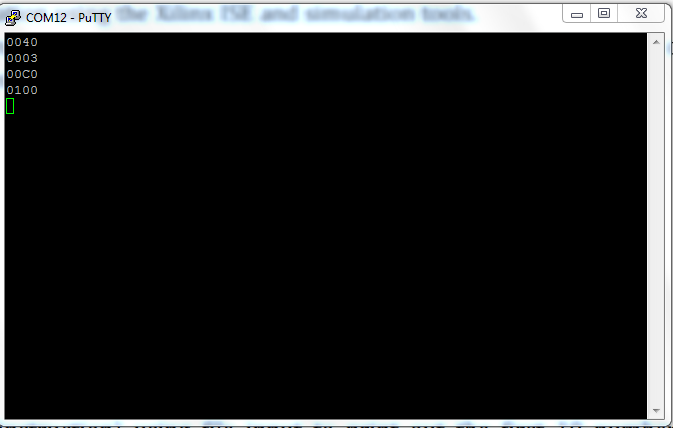
\includegraphics[width=10cm]{translation.png}
\caption{UART console output resulting from the executions in Table~\ref{table:translation}.}
\end{figure}

\section{Fibonacci}

For this section, we generated the first 10 Fibonacci numbers by writing the necessary sequencer instructions, translating them into machine instructions, and then loading them into the simulator using the \texttt{\$fopen} and \texttt{\$fscanf}.

%TODO: populate machine translations with real values

\begin{table}[H]
\centering
\begin{tabular}{ l | l }
\textbf{Sequencer Instruction} & \textbf{Binary}\\\hline
\texttt{PUSH R0 0x0} & \texttt{0101 0101}\\
\texttt{PUSH R1 0x1} & \texttt{0101 0101}\\
\texttt{SEND R0} & \texttt{0101 0101}\\
\texttt{SEND R1} & \texttt{0101 0101}\\
\texttt{ADD R0 R1 R2} & \texttt{0101 0101}\\
\texttt{SEND R2} & \texttt{0101 0101}\\
\texttt{ADD R1 R2 R0} & \texttt{0101 0101}\\
\texttt{SEND R0} & \texttt{0101 0101}\\
\texttt{ADD R2 R0 R1} & \texttt{0101 0101}\\
\texttt{SEND R1} & \texttt{0101 0101}\\
\texttt{ADD R0 R1 R2} & \texttt{0101 0101}\\
\texttt{SEND R2} & \texttt{0101 0101}\\
\texttt{ADD R1 R2 R0} & \texttt{0101 0101}\\
\texttt{SEND R0} & \texttt{0101 0101}\\
\texttt{ADD R2 R0 R1} & \texttt{0101 0101}\\
\texttt{SEND R1} & \texttt{0101 0101}\\
\texttt{ADD R0 R1 R2} & \texttt{0101 0101}\\
\texttt{SEND R2} & \texttt{0101 0101}\\
\texttt{ADD R1 R2 R0} & \texttt{0101 0101}\\
\texttt{SEND R0} & \texttt{0101 0101}\\
\texttt{ADD R2 R0 R1} & \texttt{0101 0101}\\
\texttt{SEND R1} & \texttt{0101 0101}\\
\texttt{ADD R0 R1 R2} & \texttt{0101 0101}\\
\texttt{SEND R2} & \texttt{0101 0101}\\
\texttt{ADD R1 R2 R0} & \texttt{0101 0101}\\
\texttt{SEND R0} & \texttt{0101 0101}\\
\texttt{ADD R2 R0 R1} & \texttt{0101 0101}\\
\texttt{SEND R1} & \texttt{0101 0101}\\
\texttt{ADD R0 R1 R2} & \texttt{0101 0101}\\
\texttt{SEND R2} & \texttt{0101 0101}\\
\texttt{ADD R1 R2 R0} & \texttt{0101 0101}\\
\texttt{SEND R0} & \texttt{0101 0101}\\
\texttt{ADD R2 R0 R1} & \texttt{0101 0101}\\
\texttt{SEND R1} & \texttt{0101 0101}\\
\end{tabular}
\caption{The sequencer instructions, and their corresponding machine translations, necessary to generate the first 10 Fibonacci numbers.}
\label{table:fib}
\end{table}

\begin{figure}[H]
\centering
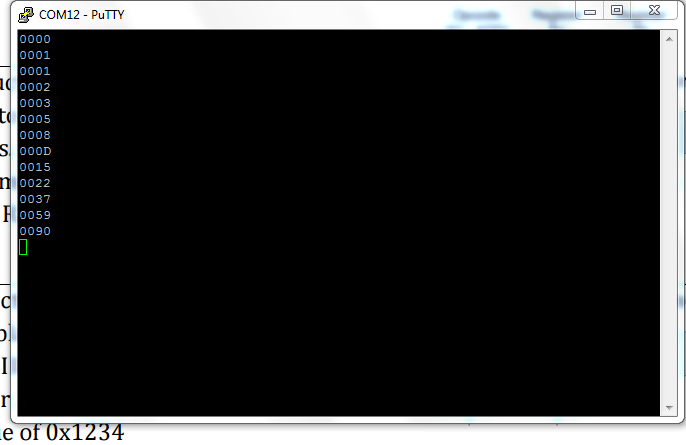
\includegraphics[width=10cm]{fib.png}
\caption{UART console output resulting from the executions in Table~\ref{table:fib}.}
\end{figure}

\section{Exercise 1}

%TODO: complete this section

\section{Exercise 2}

%TODO: complete this section

\end{document}